\documentclass[final,leqno]{siamltex1213}

\usepackage{fontspec}
\usepackage{microtype}

\usepackage{newunicodechar}
\newunicodechar{α}{\ensuremath \alpha}
\newunicodechar{β}{\ensuremath \beta}

\usepackage{amsmath}
\DeclareMathOperator{\E}{E}
\DeclareMathOperator{\Var}{Var}

\usepackage{listings}
\lstdefinelanguage{julia}{
  basicstyle=\small\ttfamily,
  showspaces=false,
  showstringspaces=false,
  keywordstyle={\textbf},
  morekeywords={if,else,elseif,while,for,begin,end,quote,try,catch,return,local,abstract,function,generated,macro,ccall,finally,typealias,break,continue,type,global,module,using,import,export,const,let,bitstype,do,in,baremodule,importall,immutable},
  escapeinside={~}{~},
  morecomment=[l]{\#},
  commentstyle={},
  morestring=[b]",
}
\lstset{language=julia, numbers=left, numberstyle=\tiny, mathescape=true}

\usepackage{todonotes}
\usepackage{algorithm}
\usepackage{algorithmic}
\bibliographystyle{siam}

\usepackage{pgfplots}
\usepackage{subcaption}

\title{Fast computation of the principal components of genomics data in Julia
    \thanks{This
        work was supported by the Intel Science and Technology Center for Big Data.
	}}

\author{%
    Jiahao Chen
    \thanks{Computer Science and Artificial Intelligence Laboratory,
           Massachusetts Institute of Technology,
           Cambridge, Massachusetts, 02139 ({\tt jiahao@mit.edu})}
    %
    \and
    Andreas Noack
    \thanks{Computer Science and Artificial Intelligence Laboratory,
            Massachusetts Institute of Technology,
            Cambridge, Massachusetts, 02139 ({\tt noack@mit.edu})}
    \and
    Alan Edelman
    \thanks{Department of Mathematics and Computer Science and Artificial Intelligence Laboratory,
            Massachusetts Institute of Technology,
            Cambridge, Massachusetts, 02139 ({\tt edelman@mit.edu})}
}


\begin{document}

\maketitle

\begin{abstract}
We describe the implementation of fast practical Lanczos algorithms employing
thick restarting and partial reorthgonalization in Julia. We present a simple
model for matrices that encode genomics data in genome-wide association studies
(GWAS), and demonstrate that Lanczos methods outperform conventionally used
software for principal component analysis of genomics matrices, such as FlashPCA.
\end{abstract}

\begin{keywords}
    singular value decomposition,
    principal components analysis,
    genome-wide association studies,
    statistical genetics,
    Lanczos bidiagonalization,
    Julia programming language
\end{keywords}

\begin{AMS}
    65F15, 97N80
\end{AMS}

\pagestyle{myheadings}
\thispagestyle{plain}
\markboth{J. CHEN, A. NOACK AND A. EDELMAN}{Principal components of genomics data in Julia}

\listoftodos

This paper is to describe the role that partial factorizations play in
organizing the various methods for doing singular value decompositions in
Julia


\section{Principal components of genome data}

Genomics data is often encoded in a matrix expressing the number of mutations
from a reference genome.
The genomics matrix is indexed by gene positions on the rows and patients on the
columns. Each matrix element counts the number of mutations a patient has from
some reference genome. Since most human cells are at most diploid, i.e.\ have
two sets of chromosomes,
the matrix elements can only be 0, 1, or 2 (or missing).

Principal component analysis has been used both to understand variation in
the statistics of human genes, as well as to correct for unwanted variations.
Perhaps most famously, principal components of human genome data have been used
to reconstruct the history of human evolution by identifying population
substructure and their relationship to other factors such as geography~\cite{Menozzi1978,Cavalli1994}
(but see \cite{Novembre2008} for criticisms of this approach).

In the context of genome-wide association studies (GWAS) for personalized
medicine, the variations due to population substructure now become confounding
factors which bias the study of which genes are correlated with desired clinical
outcomes (known as ``comorbidities'')~\cite[Ch. 8]{Laird2011}.
There are two major confounding sources of variation which are considered in
the analysis of human genome data:

\paragraph{Population stratification/admixing}
Population stratification is the phenomenon of common genetic variation within
mutually exclusive subpopulations defined along racial, ethnic or geographic
divisions~\cite{Pritchard1999,Cardon2003}. (Admixing is a relaxation of the mutual exclusion constraint~\cite{Devlin1999,Sankararaman2008}.)
In linear algebraic terms, the genomics matrix will have a low rank component
with large singular values.

\paragraph{Cryptic relatedness}
Sometimes called kinship or inbreeding, cryptic relatedness is an increase in
sampling bias in the columns (human genomes) produced by having common ancestors,
thus increasing the nominally observed frequency of certain
mutations~\cite{Voight2005,Astle2009}. Relatedness is usually detected and removed in
a separate preprocessing step~\cite{PLINK}. Any remaining related samples will
result in (near) linear dependencies in the columns of the genomic matrix,
leading to the presence of several singular values that are very small or zero.

Principal components analysis (PCA) has been proposed as a way to uncover population structure of this form~\cite{Patterson2006}.


\section{GWAS}
Genome wide association studies (GWAS) seek to associate gene variation with variations in outcome variables typically measuring a quantity related to an illness. The typical measurement for the gene variation in the genotype at different locations in the genome. Not all locations in the genome have variation in the genotype across humans so a GWAS only includes locations with variation. Locations in the genome with variation are called single nucleotide polymorphisms (SNPs) and often the explanatory data in a GWAS is simply called SNP data. The various outcome variables in a GWAS are typically called phenotypes so in short GWASs examine the relation between genotypes and phenotypes. Often in statistical studies when data is observed passively there can be doubt about the causal direction for the variables included in the analysis. However, it is generally accepted that genotypes cannot be caused by other factors included in the analysis and consequently the correlation between genotypes and phenotype could in theory be considered causal.

The genotype data is collected for a groups of individuals of varying sizes. Some studies have genotype data for hundreds of individuals but the price of sequencing genome data is rapidly declining so collection of thousands of individuals are already becoming common and it is expected that we will soon  have access to genotype data for millions of individuals.

The classical assumption in statistical studies is that the observations are randomly sampled with replacement. The reason for assumption is the implication which is that the observations can be considered independent. This might not be exactly true but should be approximately true for many statistical results to be reliable. Most collections of SNP data are from patients at a single or few hospitals in a single country. The random sampling assumption is therefore often challenged

\subsection{The model}
In a GWAS, it is customary to use a regression model for associating the genotype variation at some location in the genome and the phenotype variation. The \emph{linear} regression model can be motivated either in several different way. The readers of this will probably be familiar with the least squares formulation of the regression model which simply seeks to find the coefficients that minimize the sum of squared distances between a hyperplane and the observations. Another familiar formulation is the projection formulation where the regression problem is seen as the problem of projection a vector of observations down on the space spanned by the vectors of explanatory variables.

Statisticians are interested in quantifying the uncertainty in quantifications and consequently they introduce the regression model from probabilistic in a probabilistic setting. Statisticians will assume that the effect from genotype to phenotype can be summarized by a conditional expectation. If we for individual $i$ denote the genotype measurement by $x_i$ and the phenotype measurement by $y_i$ this can be written as $\E(y_i|x_i)=\beta_0 + \beta_1 x_i$. A popular formulation of the this model is
\begin{equation*}
    y_i = \beta_0 + x_i \beta_1 + \varepsilon_i\quad i=1,\dots,n
\end{equation*}
where $n$ is the number of observations which in this case would be the number of individuals for which we have genotype data. The variable $\varepsilon_i$ is called the error term and must satisfy $\E(\varepsilon_i|x_i)=0$. More generally, $\varepsilon_i$ is the conditional distribution $y_i - \beta_0 - x_i\beta_1|x_i$. This can also be written in matrix form

\begin{equation}
\label{eq:linreg}
    y = X\beta + \varepsilon
\end{equation}

with
\begin{equation*}
    X = \begin{pmatrix}
        1 & x_1\\
        \vdots & \vdots \\
        1 & x_n
    \end{pmatrix}
\end{equation*}

and in this notation, the well known least squares estimator can be written as
\begin{equation}
\label{eq:ols}
    \hat{\beta} = (X'X)^{-1}X'y.
\end{equation}

It might seem unnecessarily complicated to use probability theory to derive the least squares solution to the regression problem. However, when $(x_i,y_i)$ pairs are considered to be random variables then also $\hat{\beta}$ is a random variable and the mean and variance of $\hat{\beta}$ can be used to quantify uncertainty about the least square solution.

First, notice that the least squares estimator \eqref{eq:ols} can be written
\begin{equation*}
    \hat{\beta} = \beta + (X'X)^{-1}X'\varepsilon
\end{equation*}
and the expected value of the estimator is
\begin{equation}
    \E(\hat{\beta}|X) = \E(\beta + (X'X)^{-1}X'\varepsilon|X) =
        \beta + (X'X)^{-1}X'\E(\varepsilon|X) = \beta
\end{equation}
which means that the estimator is \emph{unbiased}. Statisticians are interested in the variability of $\hat{\beta}$ under changes to the data than could be considered small errors and the most common measurement for the variability of an estimator is the (conditional) variance, i.e.
\begin{equation*}
    \Var(\hat{\beta}|X) = \Var(\beta + (X'X)^{-1}X'\varepsilon|X) =
        (X'X)^{-1}X'\Var(\varepsilon|X)X(X'X)^{-1}.
\end{equation*}

This shows that variance of $\hat{\beta}$ depends on the (conditional) variance of $\varepsilon$ which hasn't been discussed yet. In classical treatments of the linear regression model it is typically assumed that, conditionally on $x_i$, the $y_i$s are independent and the have the same variance which is the same as $\Var(\varepsilon|X)=\sigma^2 I$ for some unknown scalar $\sigma^2$. Under this assumption, the variance of $\hat{\beta}$ reduces to $\sigma^2 (X'X)^{-1}$. The magnitude of this quantity is unknown because $\sigma^2$ is an unknown parameter but $\sigma^2$ can be \emph{estimated} from the data. The usual estimator is $\hat{\sigma}^2=\frac{1}{n} \|\hat{\varepsilon}\|^2$ where $\hat{\varepsilon} = y - X\hat{\beta}$. This leads to the estimate of the (conditional) variance of the estimator $\widehat{\Var(\hat{\beta}|X)} = \hat{\sigma}^2(X'X)^{-1}$.

The independence assumption is often used in statistics and can be justified from an assumption of random sampling with replacement. In studies where data is passively collected, this might not be a reasonable assumption as explained in the previous section. Non-random sampling might lead to correlation between the phenotypes even after conditioning on the genotypes. In consequence of that, $\Var(\varepsilon|X)$ will no longer be diagonal but have some general positive definite structure $\Sigma$ and $\Var(\hat{\beta}|X)=(X'X)^{-1}X'\Sigma X(X'X)^{-1}$. Since $\Sigma$ in general is consists of $\frac{n(n+1)}{2}$ parameters it cannot be estimated consistently.

In order to analyze the problem with correlated observations, it is convenient to decompose the error into a part that contains the cross-individual correlation and a part that is diagonal and therefore only describes the variance for each individual. This may be written as

\begin{equation*}
    y_i = \beta_0 + x_i\beta_1 + \eta_i + \xi_i
\end{equation*}

where is assumed that $\Var(\eta|X)=\Sigma_\eta$ and $\Var(\xi|X)=\sigma^2_\xi I$. Furthermore, it is assumes that the two error terms are independent.

\subsection{Fixed effect estimation}
A possible solution to the problem of producing a reliable estimate of the variance of $\hat{\beta}$ is to come up with a set of variables $z_1,\dots,z_k$ that proxies the correlation between the observations, i.e. $\eta=Z\gamma$. By simply including the variables $z_1,\dots,z_k$ in the regression model, it possible to remove the correlation which distorts the variance estimate for $\hat{\beta}$. For the regression $y|X,Z$, we get the least squares estimator
\begin{equation*}
    \hat{\theta} = \begin{pmatrix}\hat{\beta} \\ \hat{\gamma}\end{pmatrix} =
    \begin{pmatrix}
        X'X & X'Z \\ Z'X & Z'Z
    \end{pmatrix}^{-1}
    \begin{pmatrix}
        X' \\ Z'
    \end{pmatrix}
    (X\beta + Z\gamma + \xi)=
    \theta +
            \begin{pmatrix}
        X'X & X'Z \\ Z'X & Z'Z
    \end{pmatrix}^{-1}
    \begin{pmatrix}
        X' \\ Z'
    \end{pmatrix}\xi.
\end{equation*}
which has variance
\begin{equation*}
    \Var(\hat{\theta}|X,Z)=\sigma_\xi^2
        \begin{pmatrix} X'X & X'Z \\ Z'X & Z'Z \end{pmatrix}^{-1}
\end{equation*}.

In many applications, a few pricipal components of the covariance matrix of the complete SNP dataset is used to proxy for the correlation between individuals. Computing principal components is therefore often a first step in a GWAS. In the following section we give a brief overview over the available software for computing the principal component of SNP datasets.

\section{Software for computing the SVD of genomics data}

The software stack for GWAS is generally based on command line tools written completely in C/C++. Not only is the core computational algorithm written in C/C++ but also much of the pre- and postprocessing of the data. The datasets can be large but and the computations at times heavy but it has been a surprise to learn the extend to which analyses are carried out directly from the command line instead of using higher level languages like Matlab, R, or Python. This choice seems to limit the tools available to the analysts because, unless he is a C/C++ programmer, the programmer is restricted to the set of options included in the command line tool.

Two major packages exist for computing the PCA in the GWAS software stack. The package \emph{EIGENSOFT} accompanied~\cite{patterson2006population} which popularized the use of PCA in GWAS. In the original version of the package, the routine \texttt{smartpca} for computing the PCA of a SNP matrix was based on an eigenvalue solver from LAPACK. In consequence, all the eigenvalues and vectors of the SNP matrix were computed even though only a few of them were used as principal components. Computing the full decomposition is very inefficient and as the number of available samples has grown over the year, this approach has become impractical.

More recently, \emph{FlashPCA}~\cite{abraham2014fast}, has emerged as a potentially faster alternative to EIGENSOFT's \texttt{smartpca}. The PCA routine is based on a truncated SVD algorithm described in~\cite{halko2011finding}. More specifically, FlashPCA uses a subspace iteration scheme with orthogonalization by QR in each iteration. The convergence criterion is based on the Frobenius norm of the changes to the orthogonal basis. The QR orthogonalization step in the implementation of FlashPCA routine deviates from the algorithm in described~\cite{abraham2014fast} which only normalizes columnwise. Our conjecture was that this change was made to avoid loss of orthogonality in the subspace basis and the author of the package has confirmed this to us. In consequence, the timings in~\cite{abraham2014fast} do not correspond to the performance of the software run with default settings since the QR orthogonalization is much slower than the columnwise normalization. Furthermore, a degenerate basis might also converge much faster because it eventually just converges to the single largest eigenvalue.

\subsection{Comparing TSVD and FlashPCA}
For our synthetic dataset the time difference between the two methods is large. The initial preprocessing steps where the matrix is read and scaled contribute very little to any of the methods. For FlashPCA, the running time consists of two major components which is an initial matrix multiply, $XX'$, and the subsequent subspace iterations. By tracking the convergence criterion at each iteration it is clear that the convergence is very slow.

\begin{table}
    \caption{Running time in seconds for 41505x81700 SNP matrix}
    \centering
    \begin{tabular}{lrr}
                                   & FlashPCA & Julia Lanczos \\
        Preprocessing              &   53     & 54            \\
        Matrix multiplication      &  927     & .             \\
        Subspace/Lanczos iteration & 1639     & 37            \\
        Postprocessing             &   10     & 0             \\
        Total                      & 2629     & 81
    \end{tabular}
\end{table}

\begin{figure}
    \centering
    \begin{subfigure}{0.75\textwidth}
        \begin{tikzpicture}
            \begin{semilogyaxis}[width=10cm, height=5cm, xmin = 0, xmax = 149, ymin=10e-15, ymax=10e1]
                \addplot[very thick] file {data/FlashPCAconv.txt};
            \end{semilogyaxis}
        \end{tikzpicture}
        \caption{FlashPCA}
    \end{subfigure}
    \begin{subfigure}{0.2\textwidth}
        \begin{tikzpicture}
            \begin{semilogyaxis}[width=3cm, height=5cm, ymin=10e-15, ymax=10e1]
                \addplot[very thick] file {data/JuliaPCAconv.txt};
            \end{semilogyaxis}
        \end{tikzpicture}
        \caption{Julia-Lanczos}
    \end{subfigure}
    \caption{Convergence}
\end{figure}

Of particular interest in the use of low rank approximations for SVDS.
In this case it is not necessary to compute $U$, $S$ and $V$ and
their entirety; rather, it suffices to determine the first $k$ diagonal
entries of $S$, being the $k$ largest singular values, and their
corresponding columns of $U$ and $V$.

The Lanczos bidiagonalization~\cite{Golub1965} is a natural choice.

This paper describes an implementation of the Lanczos bidiagonalization
method written in pure Julia.

\section{Implementing simple bidiagonalization in Julia}

\begin{algorithm}
\caption{Simple Golub-Kahan-Lanczos bidiagonalization in pseudocode}

\begin{algorithmic}
\REQUIRE A matrix $A$ and a unit vector $q$
\STATE $\beta_0$ = 0
\FOR{$j=1,2,\dots,k$}

\STATE $\tilde{p}_j = A q_j - \beta_{j-1} p_{j-1}$
\STATE $\alpha_j = \left\Vert \tilde{p}_j \right\Vert_2$
\STATE $p_j = \tilde{p}_j / \alpha_j$

\STATE $\tilde{q}_{j+1} = A^\prime p_j - \alpha_j q_j$
\STATE $\beta_j = \left\Vert \tilde{q}_{j+1} \right\Vert_2$
\STATE $q_{j+1} = \tilde{q}_{j+1} / \beta_j$

\ENDFOR
\RETURN $\left(p_1, \dots, p_k, q_1, \dots, q_{k+1},\right) \alpha_1, \dots, \alpha_{k+1}, \beta_1, \dots, \beta_{k+1}$
\end{algorithmic}
\end{algorithm}



\begin{algorithm}
\caption{Simple Golub-Kahan-Lanczos bidiagonalization in Julia}

\begin{lstlisting}
function svd_gkl(A, q; maxiter=minimum(size(A)))
    m, n = size(A)
    T = eltype(A)
    Tr = typeof(one(T)/norm([one(T)]))

    $α$s = Tr[]
    $β$s = Tr[]
    P = zeros(T, m, 0)
    Q = [q]

    $β$ = zero(Tr)
    p = zeros(size(A, 1))
    for iter in 1:maxiter
        p = A*q - $β$*p
	$α$ = norm(p)
        p = p/$α$
        push!($α$s, α)
        P = [P p]

        q = A'p - $α$*q
        $β$ = norm(q)
        q = q/$β$
        push!($β$s, β)
        Q = [Q q]
    end

    B = Bidiagonal($α$s, $β$s[1:maxiter-1], true)
    F = svdfact(B)
    LinAlg.SVD(P'F[:U], F[:S], F[:Vt]*Q[:,1:maxiter]')
end
\end{lstlisting}
\end{algorithm}

Julia is a high level dynamic language for technical
computing~\cite{Bezanson2012,Bezanson2015}. While it shares superficial
syntactic similarities with other high level languages such as Matlab or
Python, Julia was designed specifically for technical computing for the ground
up, with a syntax that supports the expressiveness demanded by mathematical
notation while facilitating compiler optimizations to generate fast machine
code.

Let's explain some feature of Julia exhibited by this code listing.

\paragraph{Type arithmetic.}
This function takes as input any $A$ that supports
matrix-vector products of the form $Aq$ and $A^\prime p$. As such, the element
types of $U$, $S$ and $V$ depend on the element type of $A$.

\paragraph{Special matrix types.}
Julia's base library also supports many special matrix types, such as
\verb|Bidiagonal| for bidiagonal matrices. The \verb|Bidiagonal| constructor
seen in this code listing creates an object that represents a bidiagonal
matrix, but stores only the diagonal and its superdiagonal (the \verb|true|
argument denotes that the matrix is upper bidiagonal). The generic function
system available in Julia~\cite{Bezanson2012,Bezanson2015} allows us to define
multimethods for functions such as \verb|svdfact| for computing the SVD
factorization of a matrix, but without restricting the function to work only
on ordinary dense matrices. In fact, it is precisely the definition of a
\verb|Bidiagonal| object (called a \verb|type| in Julia) which allows us to
specify which algorithm to run.

A simplified definition of the \verb|svdfact| function in the base Julia
library looks like this:

\begin{lstlisting}
function svdfact{T<:BlasFloat}(A::StridedMatrix{T}; thin::Bool=true)
    U, S, V$^T$ = LAPACK.gesdd!(thin ? 'S' : 'A', copy(A))
    SVD(U, S, V$^T$)
end

function svdfact{T<:BlasFloat}(A::Bidiagonal{T})
    D, _, U, Vt, _, _ = LAPACK.bdsdc!(M.isupper ? 'U' : 'L',
                        'I', copy(A.dv), copy(A.ev))
    SVD(U, S, V$^T$)
end
\end{lstlisting}

The \verb|svdfact| function has two methods defined. The first defines a SVD
factorization on dense matrices as the result of LAPACK's \verb|_GESDD|
function, wrapping the output in an \verb|SVD| object. The \verb|SVD| object itself is defined as

\begin{lstlisting}
immutable SVD{T,Tr,M<:AbstractArray} <: Factorization{T}
    U::M
    S::Vector{Tr}
    V$^T$::M
end
\end{lstlisting}


annd the other on \verb|Bidiagonal| matrices. berbidiaogonal thus we
sw

\paragraph{Special factorization types.}
Low cost abstractions

\section{Practical considerations}

\subsection{Partial reorthogonalization}

\missingfigure{Code listing for reorthogonalizations}

\todo{Jiahao}

\subsection{Thick restarting}

We also implement the thick restart method for Lanczos bidiagonalization, as described in \cite{Baglama2005}.
\missingfigure{Code listing for thick restart}

\todo{Jiahao}

\section{Convergence analysis of FlashPCA}

Software like FlashPCA make use of randomized subspace interactions, which are
essentially equivalent to subspace iteration with a randomized starting subspace.

FlashPCA uses an unconventional convergence criterion, namely the matrix norm
of the difference between successive subspace basis vectors,
$\Vert Y_n - Y_{n-1} \Vert$.

By contrast, the standard measures of convergence using the residual norm yield
a simple error estimate for the uncertainty in a computed eigenvalues.

\cite[Theorem 4.5.1]{Parlett1998} states, in slightly altered notation, that for
any scalar $\theta$ and vector $v$, there is an eigenvalue $\lambda$ of $Y$ satisfying
\[
\vert\lambda - \theta\vert \le \Vert Y v - v \theta \Vert
\]

Notably, this result does not require that $(\theta, v)$ be a Ritz pair or have
any variational structure whatsoever. Therefore, we can use

\[
\Delta \sigma_i = \sqrt{\Vert X X^T v_i - v_i \theta_i \Vert}
\]

as an error bar for using $\sqrt{\theta_i}$ as an estimate for a singular value,
where $(\theta_i, v_i)$ is some eigenpair of $Q^T X X^T Q$ computed at any
iteration of FlashPCA.


\section{Results on genomics data matrix}


\subsection{The Marchenko-Pastur law}

The Marchenko-Pastur law describes the distribution of governs the eigenvalues
of a random covariance matrix $Y=XX^T$ formed from a data matrix $X$
of iid elements with mean 0 and finite variance $\sigma^2$.
Let $\rho$ be the ratio of the number of rows of $X$ to the number of columns of $X$.
Then, the nonzero eigenvalues follow the distribution
%
\begin{equation}
%    \label{eq:mplaw-ev}
    p_e(\xi) = \frac {\sqrt{(\lambda_+-\xi)(\xi-\lambda_-)}} {2 \pi \sigma^2 \lambda x}
\end{equation}
%
where
$\lambda_+ = \sigma^2(1+\sqrt{\rho})^2$ and
$\lambda_- = \sigma^2(1-\sqrt{\rho})^2$.

When written in terms of the probability density of the singular values of $X$,
the law reads
%
\begin{equation}
%    \label{eq:mplaw-sv}
    p_s(x) = \frac {\sqrt{(\sigma_+^2-x^2)(x^2-\sigma_-^2)}} {\pi \sigma^2 \min(1, \lambda) x}
\end{equation}
%
where
$\sigma_+ = \sqrt{\lambda_+} = \sigma(1+\sqrt{\rho})$ and
$\sigma_- = \sqrt{\lambda_-} = \sigma\vert1-\sqrt{\rho}\vert$.

Figure~\ref{fig:mplaw} shows typical density plots for random eigenvalues
and singular values.

% Preview source code for paragraph 0

\begin{figure}
\caption{Marchenko-Pastur law for $\rho=1.5$ (black lines) for the nonzero
eigenvalues of a random covariance matrix ($XX^{T}$) and the singular
values of $X$ for iid matrix elements with mean 0 and variance 1
(black lines). Shown for comparison are corresponding histograms (grey
bars) of numerically sampled eigenvalues and singular vectors from
a numerically sampled random matrix $X$ of size $1000\times667$,
with iid Gaussian entries of mean 0 and variance 1.
\label{fig:mplaw}
}

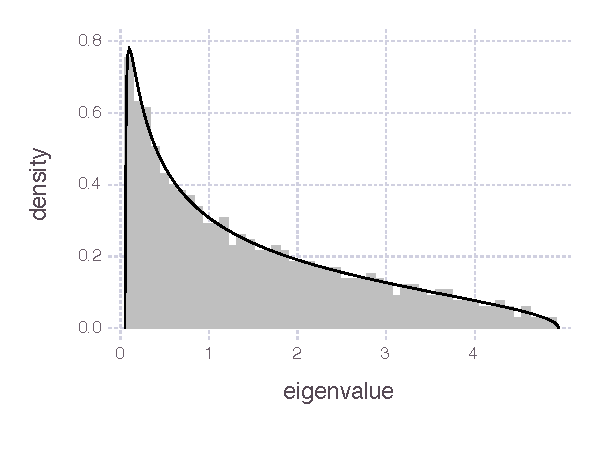
\includegraphics[width=0.45\textwidth]{fig/mplaw/fig-mplaw-ev}
%
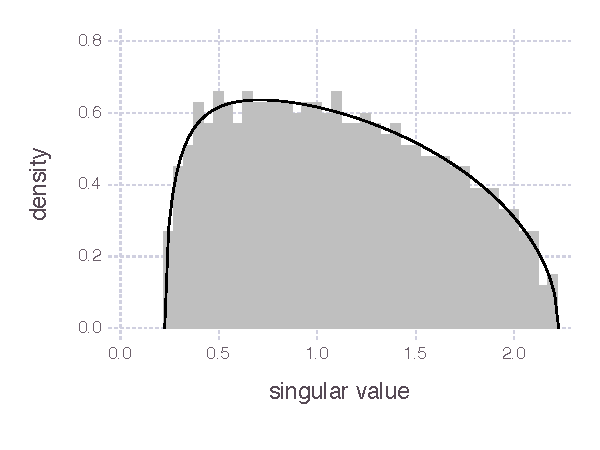
\includegraphics[width=0.45\textwidth]{fig/mplaw/fig-mplaw-sv}
\end{figure}



\subsection{Spectra of genomics matrices}

We hypothesize that the spectral properties of human patient genotype data can
be modeled the Julia code in \ref{code:model}, which captures the confounding
effects of population stratification and kinship. The former is modeled by
setting randomly select subblocks to the same value, whereas the latter is
modeled by duplicating columns, thus purposely introducing linear dependence into
the column space. This model, while simplistic, can be tuned to reproduce the
scree plot observed in empirical data matrices and we expect that such models
may be of interest to researchers developing numerical algorithms that lack
access to actual data, which are often access-restricted due to clinical privacy.

\begin{algorithm}
\caption{A simple model for human genotype data matrices in Julia
\label{code:model}}
\begin{lstlisting}
"""
Inputs:
- m: number of rows
- n: number of columns
- r: number of subblocks to model population stratification
- nsignal: number of entries to represent signal
- rkins: fraction of columns to duplicate

Output:
- A: a dense matrix of size m x n with matrix elements 0, 1 or 2
"""
function model(m, n, r, nsignal=round(Int,√(m*n)), rkins)
    A = zeros(m, n)
    #Model population stratification
    #by randomly setting a subblock to the same value, k
    for i=1:r
        k = rand(0:2)
        i1, i2 = randrange(m)
        j1, j2 = randrange(n)
        A[i1:i2, j1:j2] = k
    end

    #Model signal
    for i=1:nsignal
        A[rand(1:m), rand(1:n)] = rand(0:2)
    end

    #Model kinship by duplicating columns
    nkins = round(Int, rkins*n)
    for i=1:nkins
        A[:, rand(1:n)] = A[:, rand(1:n)]
    end
    A
end

function randrange(n)
    i1 = rand(1:n)
    i2 = rand(1:n)
    if i1 > i2
        return i2, i1
    else
        return i1, i2
    end
end
\end{lstlisting}
\end{algorithm}

The scree plot of a genomics matrix

\begin{figure}

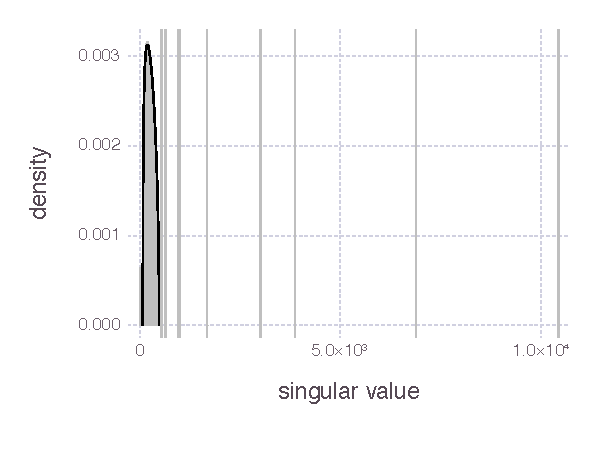
\includegraphics[width=0.5\textwidth]{fig/synthetic/fig-empirical-density}
%
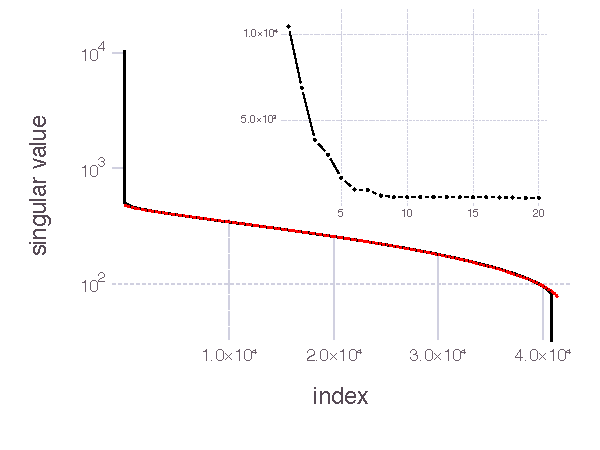
\includegraphics[width=0.5\textwidth]{fig/synthetic/fig-empirical-scree}

\caption{Left: Histogram of the singular values of a synthetic genomics data
matrix of size $81700\times41505$ (grey bars), overlaid with the Marchenko-
Pastur law for $\rho = 1.86$ (black line). Light grey vertical lines show the
presence of 18 outlying singular values whose magnitudes exceed
$1.1\sigma_+ \approx 529.7$.
Right: Scree plot of the singular values of the same matrix
(black solid lines), showing the presence of a large, low rank portion
of approximately rank 10 (inset), and an asymptotic convergence to the same
Marchenko-Pastur law (red dotted line).}
\label{fig:scree}
\end{figure}

Random matrix theory was previously introduced in the theoretical analysis of
principal components of genomics matrices. \cite{Patterson2006} proposed a
hypothesis test that computed principal components should correspond to eigenvalues
that were different from those expected from a pure random covariance matrix,
and comparing in particular the largest eigenvalue against one randomly sampled
from the Tracy-Widom distribution~\cite{Tracy1993,Tracy1994}.
Here, we make the further observation that the bulk distribution must further satisfy the Marchenko-Pastur law~\cite{Marchenko1967}.


\subsection{Accuracy and speed results}

\begin{table}
\begin{tabular}{|c|c|c|c|c|c|c|c|c|}
\hline
 & Algorithm & mvps & Wall time & $\beta_{final}$ & $\left\Vert \Delta\theta\right\Vert _{1}$ & $\left\Vert \Delta\theta\right\Vert _{\infty}$\tabularnewline
\hline
\hline
FlashPCA1 & Block power & 2280 & 2616.1 sec. & 6.4 & $4\times10^{+4}$ & $4\times10^{+4}$\tabularnewline
\hline
FlashPCA2 & Block power &  &  &  &  & \tabularnewline
\hline
PROPACK & GKL (PRO, NR) & 298 & 264.6 & - & $4\times10^{-8}$ & $4\times10^{-8}$\tabularnewline
\hline
ARPACK & GKL (FRO, IR) & 355 & 858.5 & 7.8 & $6\times10^{-3}$ & $1\times10^{-3}$\tabularnewline
\hline
this work & GKL (FRO, TR) & 280 & 397.8 & 6.4 & $2\times10^{-3}$ & $2\times10^{-3}$\tabularnewline
\hline
this work & GKL (PRO, NR) & 321 & 302.4 & 15072 & $6\times10^{-4}$ & $6\times10^{-4}$\tabularnewline
\hline
\end{tabular}

\caption{Comparing various methods for computing the top 20 principal
components on a simulated genotype matrix of size $80000\times40000$.
Linear algebra kernels were run on OpenBLAS v0.2.18 with 16 software threads.
FlashPCA1 - Reimplementation in pure Julia of the published version of FlashPCA,
FlashPCA2 - Reimplementation in pure Julia of the master version of FlashPCA available on GitHub,
GKL - Golub--Kahan--Lanczos bidiagonalization,
PRO - partial reorthogonalization,
FRO - full reorthogonalization,
NR - no restart,
IR - implicit restart after 40 Lanczos vectors,
TR - thick restart after 40 Lanczos vectors,
mvps - number of matrix--vector products.
Termination criterion set to $\Vert Y\Vert = 10^{-8}$ for FlashPCA$n$,
and relative error in the singular values of $10^{-8}$ for the Lanczos methods.
}
\end{table}

\begin{figure}
\caption{Convergence behavior of thick-restarted Lanczos with full reorthogonalization, with top 20 singular values requested. Restarts were triggered every 40 microiterations (grey vertical lines).
\label{fig:lanczos-tr}
}

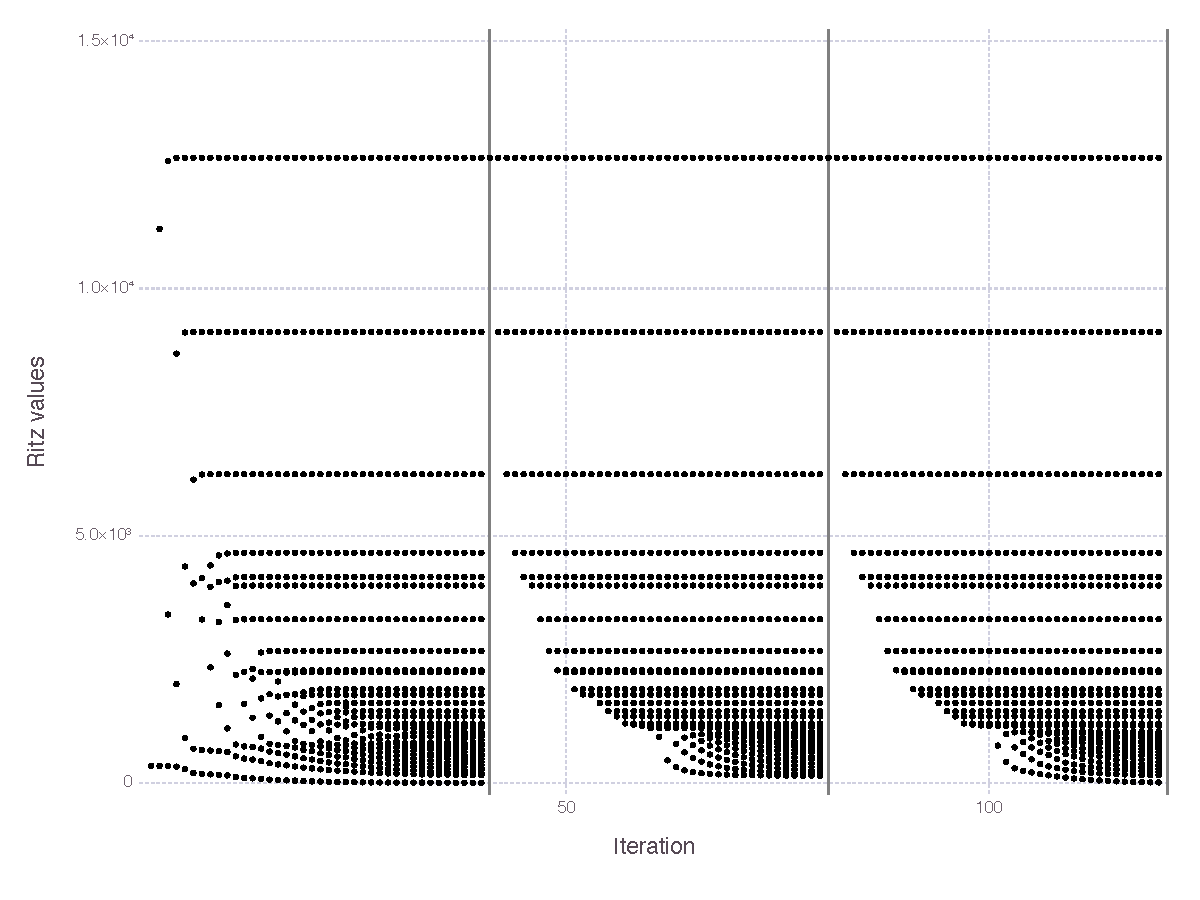
\includegraphics[width=\textwidth]{fig/thickrestarted/fig-conv}
\end{figure}



\section{Conclusions}



\section*{Acknowledgments}

We thank the Julia development community for their contributions to free and
open source software. Julia is free software that can be downloaded from
\url{julialang.org/downloads}. The implementation of iterative SVD described in
this paper is available as the \verb|svdl| function in the
\href{IterativeSolvers.jl}{https://github.com/JuliaLang/IterativeSolvers.jl}
package. J.C. would also like to thank Jack Poulson (Stanford), David Silvester
(Manchester), and Alex Townsend (MIT) for many insightful discussions.

\bibliography{bio,svd}

\end{document}
